\section{Noise reduction in the frequency domain}

\subsection{The Fourier spectra of a noisy image and the original image}

\begin{figure}[ht]
\centering
	\subfigure[Base Lena image]{
	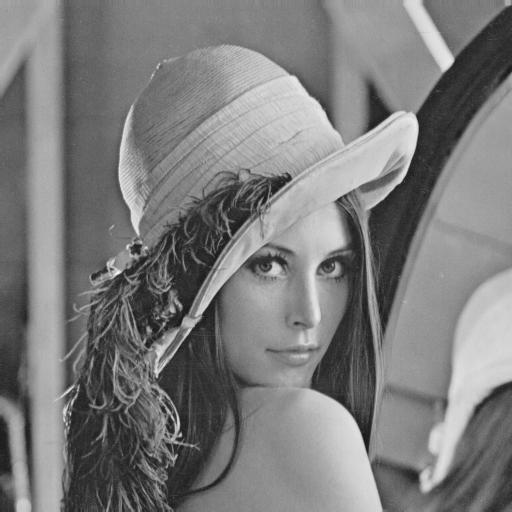
\includegraphics[width=0.45\textwidth]{question5/1_lenaBase}
	}
	\subfigure[Log Fourier spectrum]{
	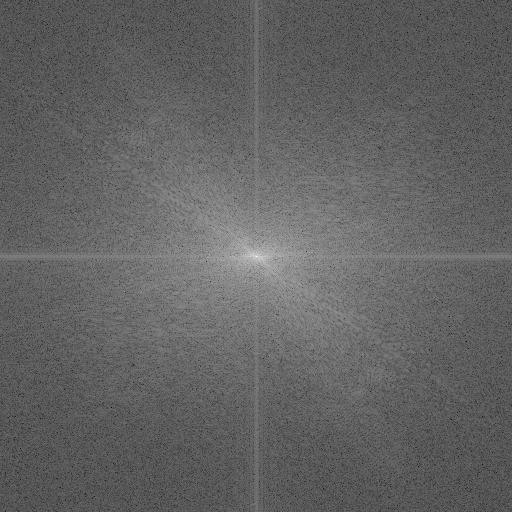
\includegraphics[width=0.45\textwidth]{question5/1_lenaBase_fft}
	}
	\subfigure[Lena image with Gaussian noise, $\sigma^2$=0.005; PSNR +23.02dB]{
	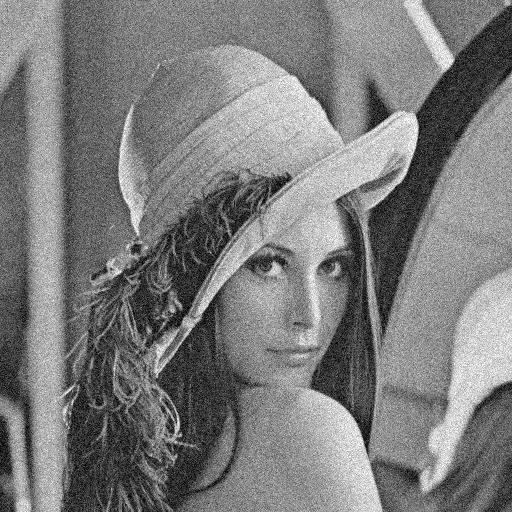
\includegraphics[width=0.45\textwidth]{question5/1_lenaNoisy}
	}
	\subfigure[Log Fourier spectrum]{
	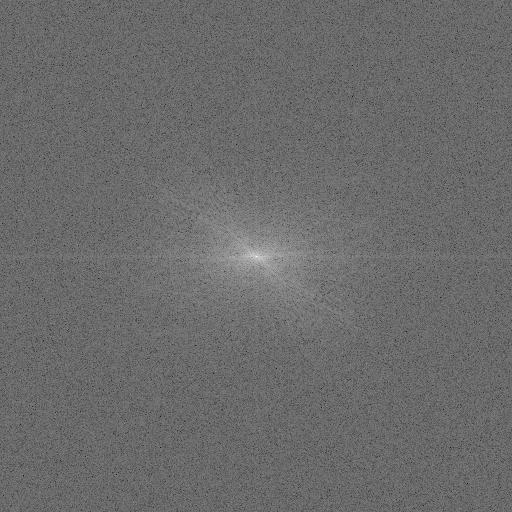
\includegraphics[width=0.45\textwidth]{question5/1_lenaNoisy_fft}
	}
\end{figure}

\subsubsection{Compare the two Fourier spectra. What are the differences? Where is these differences most visually
prominent? Why?}

The noisy Fourier spectrum looks like a reduced contrast version of the original Fourier spectrum. This is because the Gaussian noise is uniformly applied across all frequencies, so the contrast of the Fourier spectrum is decreased. These differences are most prominent in the high frequency areas of the Fourier spectra as most photographs contain most of their detail in the low frequencies; while Gaussian noise is uniform in the Fourier domain.


\subsection{Low-pass filtering with a cutoff of 60}
\begin{figure}[ht]
\centering
	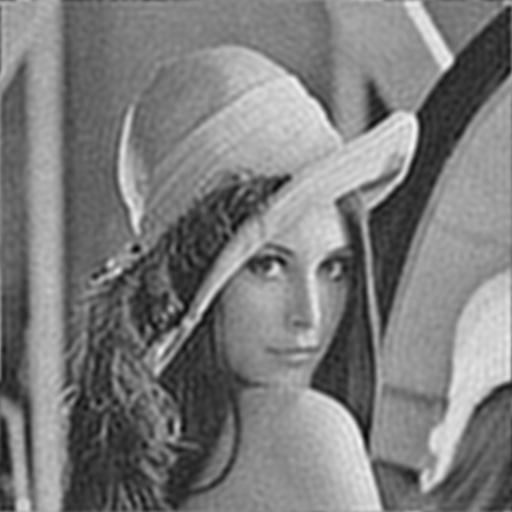
\includegraphics[width=0.45\textwidth]{question5/2_lena_LFP_60}
	\caption{Image filtered using low-pass with a cutoff of 60; PSNR +27.90dB}
\end{figure}

\subsubsection{Describe the appearance of the denoised image compared to the original and the noisy images. Why does it look this way? What does the ideal low-pass filter do?}

The ideal low-pass filter averages out the noise in the image, reducing the noise's effects. The image looks like a slightly blurred version of the original image. As the noise is uniformly distributed and the image details are mostly concentrated in the lower frequencies, the filter reduces the high frequency noise in the image.

\subsubsection{There is a particular artifact present in the restored image. What is it and why does it happen?}

The restored image has a slight ringing effect. This artifact occurs because the inverse Fourier transform of the ideal disc cutoff is a sinc function. This causes ringing artifacts at areas with a transition between colours, as demonstrated around the top left edge of the bowl of Lena's hat.

\subsection{Low-pass filtering with a cutoff of 20}
\begin{figure}[ht]
\centering
	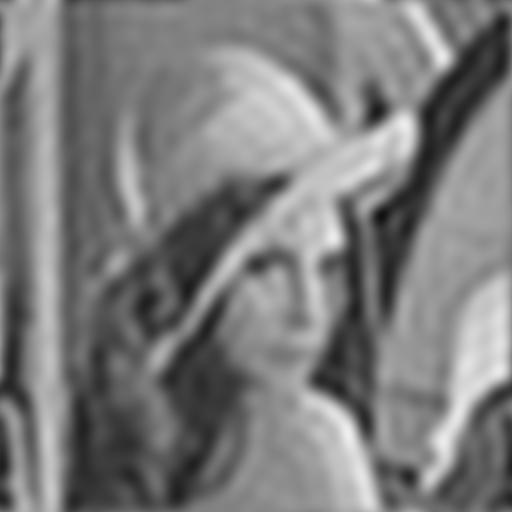
\includegraphics[width=0.45\textwidth]{question5/3_lena_LFP_20}
	\caption{Image filtered using low-pass with a cutoff of 20; PSNR +23.11dB}
\end{figure}

\subsubsection{Compare the denoised image with the denoised image using a cut-off radius of 60. How does the
image and the PSNR differ? Why?}

This denoised image is much blurrier than the image with a cutoff radius of 60. The ringing artifacts are also much more pronounced, and are visible without zooming in on the image.This results in a much lower PSNR. 

By setting the cutoff frequency so low, many of the high frequency details of the original image are filtered out, such as the features of Lena's face and the feathers in the image. When examining the Fourier spectra of the original image, there still do exist many image components that would be outside the radius 20 cutoff, so image information is excessively attenuated.

\subsubsection{What conclusions can you draw about the relationship between cut-off radius and resulting image after filtering? What is the trade-off in terms of noise reduction?}

Decreasing the cut-off radius will reduce the number of high frequency components included in the output image. As image components tend to be concentrated in low frequency areas and noise is uniformly distributed, this has the effect of reducing noise.

If the cut-off radius is excessively decreased, some of the mid-high frequency components of the image will also be attenuated, reducing the sharpness of the image. When reducing noise in an image, one must always be mindful not to excessively smooth the image resulting in an excessive loss of sharpness in the image (and also leading to ringing artifacts).

\clearpage
\subsection{Using a Gaussian low-pass filter}

\subsubsection{Compare the denoised image with the denoised images produced using the ideal low-pass filters. How does the image and the PSNR differ? Is it better or worse? Why? Does it have the same type of image artifacts?}

The denoised image using a Gaussian low-pass filter looks very close to the original image. It performs better because the Fourier transform of a Gaussian is also a Gaussian, which allows the filter to reduce ringing artifacts. The Gaussian also manages to better retain the high frequency detail in the image. Instead of removing all high frequency components, the Gaussian drops off slower. While this preserves some noise, it tends to retain more details as well.


\begin{figure}[ht]
\centering
	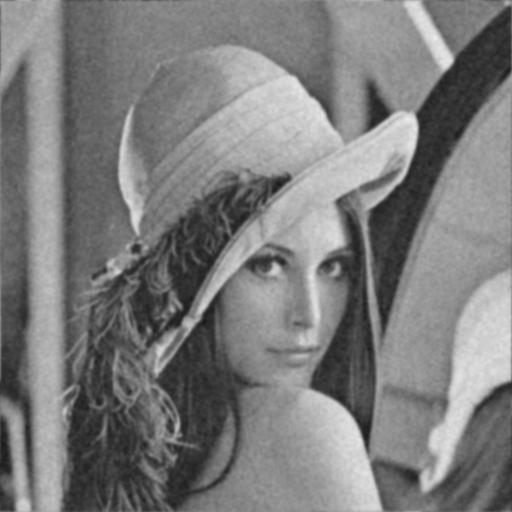
\includegraphics[width=0.45\textwidth]{question5/4_lena_LFP_gauss60}
	\caption{Image filtered using Gaussian low-pass filter, $\sigma^2$=60; PSNR +29.53dB}
\end{figure}